\section{The Margin Over a Prompt Is Not Monotone in Capability}
\label{app:interaction}

\begin{figure}[htbp]
\centering
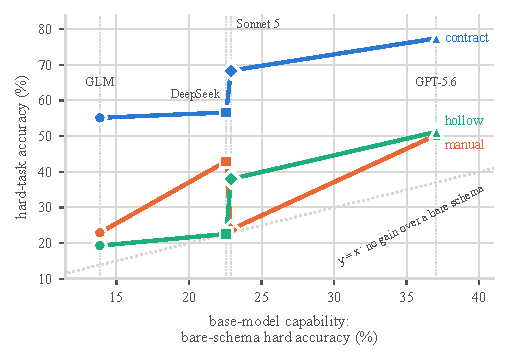
\includegraphics[width=\columnwidth]{figures/fig-interaction.pdf}
\caption{Hard accuracy against base-model capability, where capability is
the bare-schema arm's own accuracy. The margin over \armM{} is $+32.2$,
$+13.7$, $+44.6$ and $+27.1$: not monotone.}
\label{fig:interaction}
\end{figure}

Ordered by what each model achieves from a bare schema
(Figure~\ref{fig:interaction}), the contract's margin over \armM{} on hard
tasks runs $+32.2$, $+13.7$, $+44.6$ and $+27.1$ on \mGLM{}, \mDS{},
\mSON{} and \mGPT{}. With the two flash models alone the pattern reads
as a clean interaction: \armM{} improved by 20.0 points while \armC{} moved 1.5,
and the lines converged. Two readings were available. Structured context
might substitute for capability, so that a stronger model extracts the same
semantics from prose unaided and the margin keeps shrinking; or \armC{}
might have been pinned near a benchmark ceiling at ${\approx}56\%$ while
\armM{} rose to meet it. \mGPT{} reached 77.4\%, so there is no ceiling at
56\%, and its $+27.1$ refutes the shrinking margin; \mSON{}'s $+44.6$ is the
largest of the four, on a model whose bare-schema score ties \mDS{}'s.
Whatever governs the size of the contract's advantage over a hand-written
prompt, it is not a monotone function of base capability, and four points
cannot support a third story. \mSON{} adds one thing: the bare-schema score
is a poor proxy for what a model does with structure. \mSON{} and \mDS{} are
0.3 points apart on it and 11.8 points apart with the contract.
